\documentclass[11pt, oneside]{article}     % use "amsart" instead of "article" for AMSLaTeX format
\usepackage{geometry}                		% See geometry.pdf to learn the layout options. There are lots.
\geometry{letterpaper}                   		% ... or a4paper or a5paper or ... 
%\geometry{landscape}                		% Activate for for rotated page geometry
%\usepackage[parfill]{parskip}    		% Activate to begin paragraphs with an empty line rather than an indent
\usepackage{graphicx}				% Use pdf, png, jpg, or epsß with pdflatex; use eps in DVI mode
								% TeX will automatically convert eps --> pdf in pdflatex		
\usepackage{amssymb}
\newcommand{\pr}{\mathrm{P}}
\renewcommand{\vec}[1]{\mathbf{#1}}

\title{A Sampling of Ideas}
\author{Bill DeRose
\\ Advisor: Gabe Chandler}


\usepackage{Sweave}
\begin{document}
\Sconcordance{concordance:thesis_topic_1.tex:thesis_topic_1.Rnw:%
1 16 1 1 0 36 1 1 10 9 0 1 19 20 0 1 3 5 0 1 2 2 1}

\maketitle
\section{Introduction}
The  difficulties we face in computational statistics are a consequence of modern technology.
%It is a consequence of modern technology that we face computational difficulties in the field of statistics. 
We should be so lucky to face the problem of designing algorithms to generate truly random numbers. And yet, we delude ourselves into believing there is randomness where there is none.

_
The image on the left is genuine randomness, while the image on the right is too evenly spaced for it to be \emph{truly} random. In actuality, the left plots star locations while the right depicts the positions of glowworms on the ceiling of a cave in New Zealand. The glowworms spread themselves out evenly to reduce competition for food amongst themselves; the even distribution is the result of a non-random force. The right image suggests true randomness appears in clusters.

In our study of sampling methods, we assume the existence of a random
number generator that allows us to sample $U \sim \mbox{Unif}(0,1)$. From this, we explore
the techniques and methods that allow us to sample from more complex distributions. We begin with a
review of classical sampling (simple sampling, rejection sampling, importance sampling) before directing the majority of our attention to Monte Carlo based methods. In specific, we explore the advantages of Hamiltonian and gradient based Monte Carlo over traditional Markov Chain Monte Carlo simulations.
By treating the state space as a dynamical system, we may apply Hamiltonian dynamics to 
explore the target distribution more efficiently. However, before we embark on the discussion of gradient methods, we discuss the classical Markov Chain Monte Carlo algorithm and its application to sampling from high-dimensional distributions. 
\subsection{Markov Chain Monte Carlo}
Although the sampling techniques we have discussed worked well, they required us to 
have a closed form cdf of the target distribution. As we will see, the previous approaches also fail as we move to higher dimensional space and the curse of dimensionality sets in. We turn to Markov Chain Monte Carlo simulations because they ameliorate many of the problems faced by classical sampling.


A Monte Carlo simulation allows us to approximate the probability of certain outcomes by running a large number of
trials to obtain an empirical distribution of possible events. A Markov chain is a series of random variables 
$\vec{x}^{(1)}, \ldots, \vec{x}^{(m)}$ such that
\begin{equation}
\pr(\vec{x}^{(m + 1)} | \vec{x}^{(m)}, \vec{x}^{(m-1)}, \ldots, \vec{x}^{(1)}) =\pr(\vec{x}^{(m + 1)} | \vec{x}^{(m)}) 
\end{equation}
Markov Chain Monte Carlo simulations use Markov chains whose stationary (equilibrium) distribution we wish to sample from. By initializing the Markov chain with an initial state and transition probabilities, we may run the chain for a ``sufficient" number of steps to draw samples from the desired distribution. It is common to ignore some number of samples at the beginning (burn-in), and then consider only every $n^{{th}}$ sample when computing an expectation.

Below is an implementation of such a Markov Chain Monte Carlo sampler, a Gibbs 
Sampler which will sample from a 2D exponential.
\begin{Schunk}
\begin{Sinput}
> Exp.Bounded <- function(rate, B) {
+   # rexpT samples from the exponential distribution
+   # until a value less than B is observed
+   x <- rexp(1, rate)
+   while (x > B) {
+     x <- rexp(1, rate)
+   }
+   return(x)
+ }
> Gibbs.Sampler <- function(M, B) {
+   # Gibbs.Sampler uses the Gibbs sampling method
+   # to sample from a joint distribution given our
+   # knowledge of the condition distributions.
+   mat <- matrix(ncol=2, nrow = M)
+   x <- 1
+   y <- 1
+   mat[1, ] <- c(x, y)
+   for (i in 2:M) {
+       x <- Exp.Bounded(y, B)
+       y <- Exp.Bounded(x, B)
+       mat[i,] <- c(x, y)
+   }
+   layout(matrix(c(1,1,2,3), 2, 2, byrow = TRUE))
+   plot(mat, main="Joint Distribution", xlab="X",ylab="Y")
+   hist(mat[ , 1], main="Marginal dist. of X", xlab="X")
+   hist(mat[ , 2], main="Marginal dist. of Y", xlab="Y")
+ }
\end{Sinput}
\end{Schunk}
\begin{Schunk}
\begin{Sinput}
> Gibbs.Sampler(1000, 10)
\end{Sinput}
\end{Schunk}
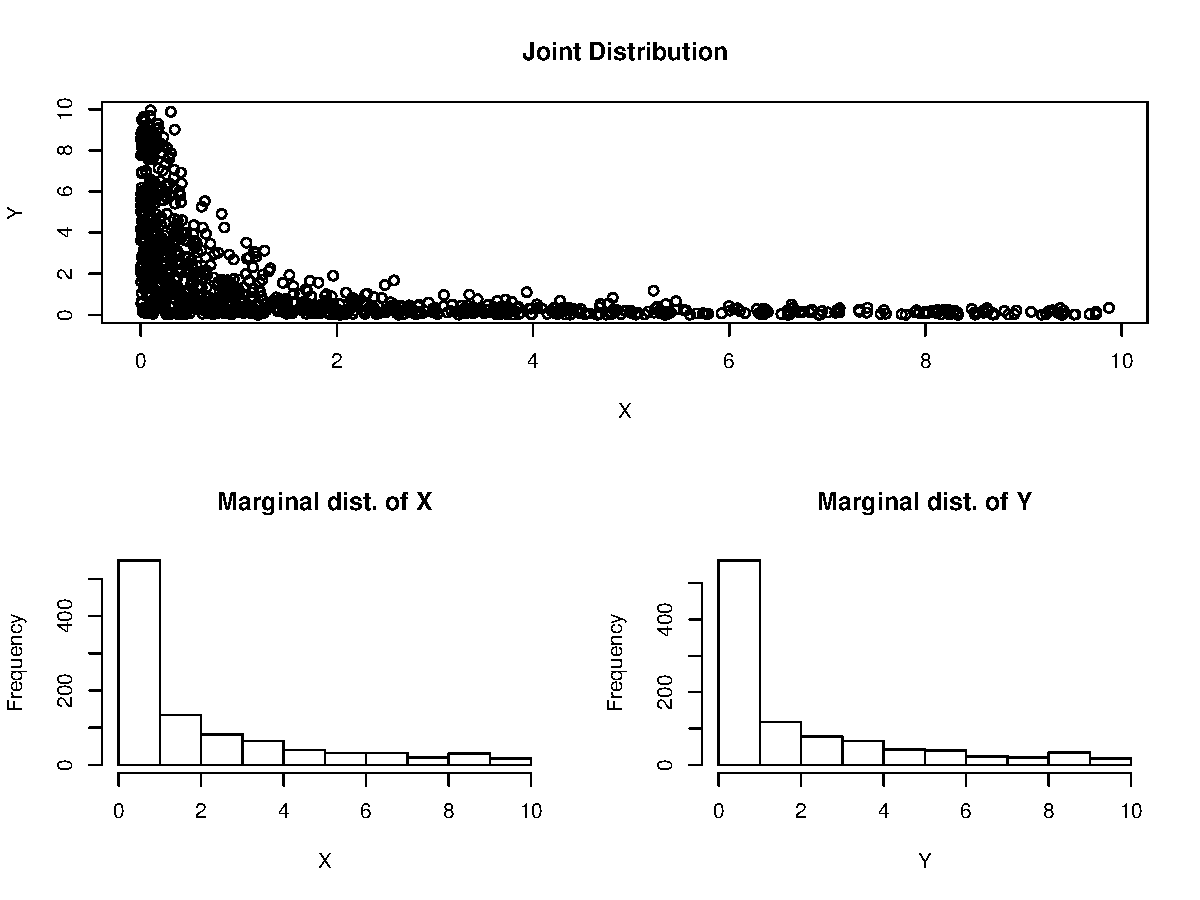
\includegraphics{thesis_topic_1-gibbsSampler}


\end{document}
